\section{Returns time series simulations}
\label{sec:simulations}

In Sect. \ref{subsec:gauss_alg_sim} we simulate returns time series following
a multivariate Gaussian and algebraic distribution. We test the influence of
the normalization within the epochs in the ergodicity defect in Sect.
\ref{subsec:norm_epochs_sim} and propose a solution for this defect in Sect.
\ref{subsec:norm_full_sim}. Finally we use empirical data to support our
simulation findings in Sect. \ref{subsec:emp_results}.

%%%%%%%%%%%%%%%%%%%%%%%%%%%%%%%%%%%%%%%%%%%%%%%%%%%%%%%%%%%%%%%%%%%%%%%%%%%%%%%
\subsection{Simulation of multivariate Gaussian and algebraic distributions}
\label{subsec:gauss_alg_sim}

In Sect. \ref{subsubsec:gauss_sim} we describe the methodology to simulate
multivariate Gaussian distributed returns time series and in Sect.
\ref{subsubsec:alg_sim} we describe the methodology to simulate multivariate
algebraic distributed returns time series.

%%%%%%%%%%%%%%%%%%%%%%%%%%%%%%%%%%%%%%%%%%%%%%%%%%%%%%%%%%%%%%%%%%%%%%%%%%%%%%%
\subsubsection{Multivariate Gaussian distributions}\label{subsubsec:gauss_sim}

To simulate the returns time series, we use a method \cite{drawing_dist} for
drawing a random vector $x$ from the $N$-dimensional multivariate Gaussian
distribution with mean vector $\mu$ and covariance matrix $\Sigma$. First, we
create a correlation matrix $C$ with $c = 1$ on its diagonal and $c = 0.3$ on
its non-diagonal entries. Then, we compute the eigenvalues and eigenvectors
of the correlation matrix, such that $\Sigma = U \Lambda U^{-1}$. We get a $z$
vector whose components are drawn from a independent standard Gaussian
distribution. Finally we obtain the returns with the desired distribution as
\begin{equation}
    r = \mu + U \Lambda^{1/2} z
\end{equation}

In our case, the $r$ vector components are drawn from a normal distribution
with covariance matrix $\Sigma$ and $\mu$ vector zero.
With these method we want to obtain time series simulating the data matrix G
with dimensions $2 \times T$, where $T$ is the window length of the epochs.
These returns can be later rotated and aggregated to compare with the behavior
of the results in Sect. \ref{subsec:epochs}.
The goal of this approach is that all simulations should show standard normal
distributions.

With the simulated pair returns time series, we proceed to local normalize the
epoch, we evaluate the $2 \times 2$ sample covariance matrix and diagonalize
it. We rotate the two-component returns vectors into the eigenbasis of the
correlation matrix and normalize the axis with the eigenvalues. Finally we
aggregate all the components into a single univariate distribution.

\begin{figure}[htbp]
    \centering
    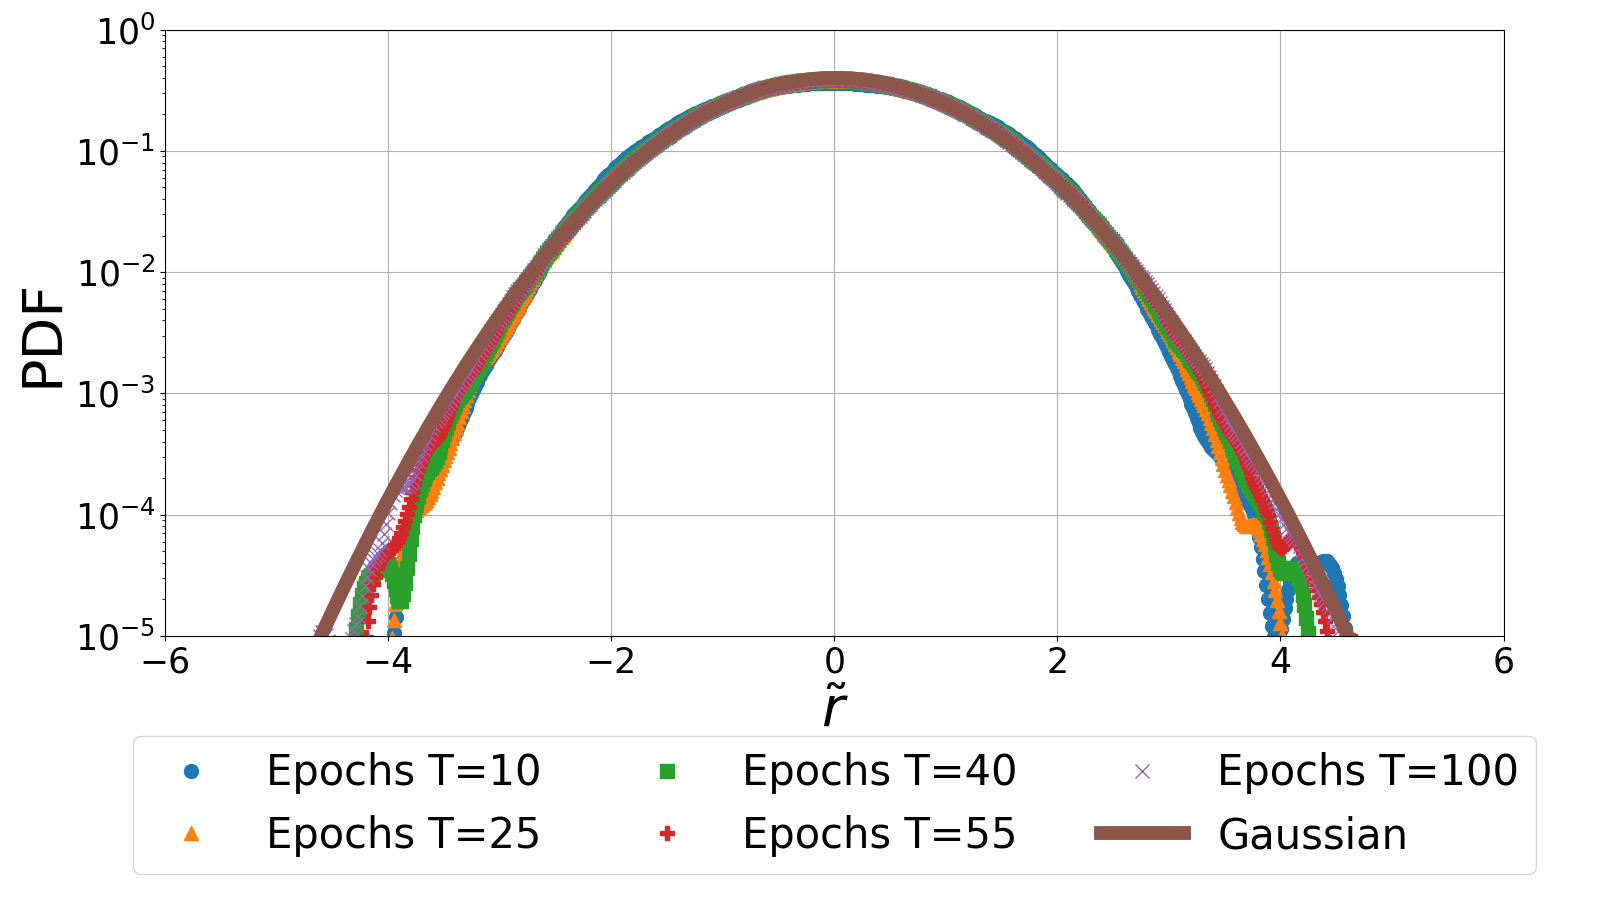
\includegraphics[width=0.6\columnwidth]
    {figures/06_epochs_sim_agg_ret_pairs_no_norm.png}
    \caption{Simulated aggregated rotated and scalated distribution of returns
             ($\tilde{r}$) for fixed covariance and $K=50$ without
             normalization within the epochs. $\Delta t = 1$ unit and epochs
             window  lengths $T=10, 25, 40, 55, 100$ units.}
    \label{fig:epochs_agg_ret_pairs_no_norm}
\end{figure}

In Fig. \ref{fig:epochs_agg_ret_pairs_no_norm} we simulate time series for
$K = 50$. Each time series is made of $100$ epochs. We use epochs window
lengths $T = 10, 25, 40, 55$. As expected, as we drawn the original returns
from a Gaussian distribution with covariance matrix $\Sigma$ and $\mu$ vector
zero, all the simulations show standard Gaussian distributions. Thus, this is
our reference to check what is introducing the ergodicity effect in the 
original method.

%%%%%%%%%%%%%%%%%%%%%%%%%%%%%%%%%%%%%%%%%%%%%%%%%%%%%%%%%%%%%%%%%%%%%%%%%%%%%%%
\subsubsection{Multivariate algebraic distributions}\label{subsubsec:alg_sim}

%%%%%%%%%%%%%%%%%%%%%%%%%%%%%%%%%%%%%%%%%%%%%%%%%%%%%%%%%%%%%%%%%%%%%%%%%%%%%%%
\subsection{Normalization within the epochs}
\label{subsec:norm_epochs_sim}

Now, to check the normalization within the epochs, we simulate the returns,
normalize each epoch to mean $\mu = 0$ and $\Sigma^{1} = 1$ and finally repeat
the procedure of rotate, scale and aggregate.

\begin{figure}[htbp]
    \centering
    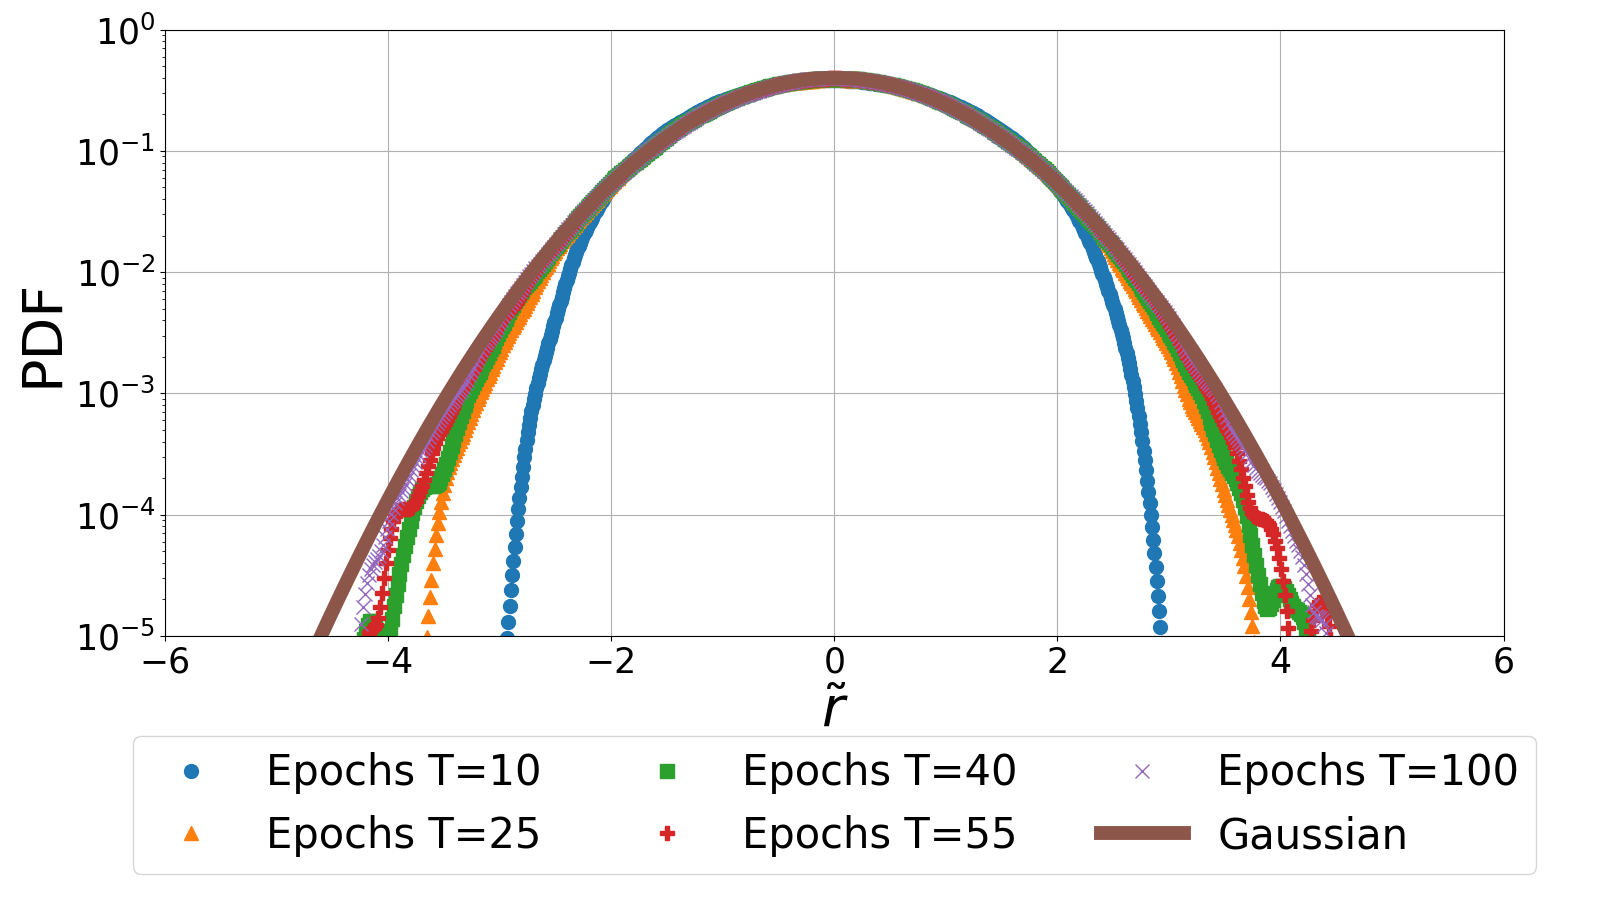
\includegraphics[width=0.6\columnwidth]
    {figures/06_epochs_sim_agg_ret_pairs_norm.png}
    \caption{Simulated aggregated rotated and scalated distribution of returns
             ($\tilde{r}$) for fixed covariance and $K=50$ with normalization
             within the epochs. $\Delta t = 1$ unit and epochs window  lengths
             $T=10, 25, 40, 55, 100$ units.}
    \label{fig:epochs_agg_ret_pairs_norm}
\end{figure}

As we can see in Fig. \ref{fig:epochs_agg_ret_pairs_norm}, the ergodicity
defect clearly appears for an epoch window length $T = 10$. As the epoch window
length grows, the ergodicity defect starts to dissapear. We could even argue,
that with a epoch window length greater or equal to $T = 25$, we already are
close enough to the Gaussian distribution, which were the objective of these
simulations. Furthermore, with large epoch windows lengths we can confirm that
the ergodicity defect disappear, as it can be seen with $T = 100$

%%%%%%%%%%%%%%%%%%%%%%%%%%%%%%%%%%%%%%%%%%%%%%%%%%%%%%%%%%%%%%%%%%%%%%%%%%%%%%%
\subsection{Normalization complete return time series}
\label{subsec:norm_full_sim}

%%%%%%%%%%%%%%%%%%%%%%%%%%%%%%%%%%%%%%%%%%%%%%%%%%%%%%%%%%%%%%%%%%%%%%%%%%%%%%%
\subsection{Empirical results}
\label{subsec:emp_results}